\section{Introduction}

The distribution of wealth and income has recently made a comeback to the
centre of economic discourse in advanced economies. The ongoing rise of
income inequality, observed since the early 1980s especially in Anglo-Saxon
countries, has received renewed attention in the public sphere since the
financial started taking its toll on living standards across the world. At
the same time, the best-selling book by \citet{Piketty2014} led to a surge
in interest in the role of capital in the economy, and, by extension, the
distribution of wealth, both in the academic literature and the popular
press. \\
While the broader public has only recently picked up on the issues arising
around income and wealth distributions, they have sat squarely in the centre
of many sub-fields of economics for a long time. The income distribution has
long been of interest to labour economists trying to understand the forces
shaping the evolution of earnings in the labour market, while at least the
accumulation of aggregate wealth plays a central role in macroeconomic
models of economic growth. This chapter, as well as chapter three, 
focuses on the intermediate step that takes us from an
income to a wealth distribution - economic models of household saving.
When attempting to build a model of the wealth distribution, the first
step of course is to get an understanding of the object we want to model.
To this end, this chapter starts by presenting stylised facts of the wealth
distributions in advanced countries and discusses some of the limitations
of the data available. It then builds a simple life-cycle model of consumption
and savings to guide the following discussion and fix notation. Using this
basic model, different savings motives and their importance in the context
of aggregate wealth accumulation are discussed. Following this, the role of
income uncertainty and market structure is examined in more detail.


\section{Stylised facts}
The most notable and consistent fact that emerges when looking at wealth
distributions across all countries and different time periods is that wealth
is highly unevenly distributed, much more so than income. This can be readily
seen when comparing Gini indices and top shares of income and wealth, as in
Table \ref{tab:gini_topshares} or looking at histograms and cdfs of wealth and
income distributions as in Figure \ref{fig:was_wealthholdings}. It is important to note
that in producing these aggregate numbers and figures, one necessarily has
to make decisions on how exactly to construct measures of income and wealth,
which will have to be kept in mind when comparing model predictions with
empirical numbers. When constructing an income measure, the obvious starting
point are labour earnings, and for many economic applications simply
observing an individual's wages will be enough. When thinking about questions
of consumption smoothing though, we are ultimately interested in accounting
for all claims on consumption goods available to an individual or household
in a given period, and while for most people the largest part of these claims
stem from labour earnings, we will also want to account for the effect of
government programs (by constructing a post-tax, post-transfer income measure),
income from accumulated assets, and potentially even informal insurance
arrangements such as inter-vivos transfers between family and friends.
In constructing wealth measures, we again have to think closely about the
question we are trying to answer when constructing them. If the goal is to
account for all productive capital in the economy that can be used in
production, a measure of total net wealth aggregating all forms of asset and
debt classes, and including some durable consumption goods such as cars. When
thinking about the role of wealth in helping the household to smooth out
income fluctuations, it might be more appropriate to exclude very illiquid
assets such as housing, and look more closely at the role of debt for households
which might be at their borrowing constraint and are thus vulnerable to
reductions in their borrowing limit, even though their net wealth (including
illiquid assets) is positive. Finally, important questions are raised by
the existence of various government and private pension schemes, which have
to be factored in when constructing measures of a household's lifetime
resources, but whose exact value might be uncertain (for the case of defined
contribution plans) and not well understood by households themselves.


\begin{table}%
\begin{tabular}{lcr}

\end{tabular}
\caption{Measures of wealth concentration in different data sets.}
\label{tab:gini_topshares}
\end{table}

\begin{figure}
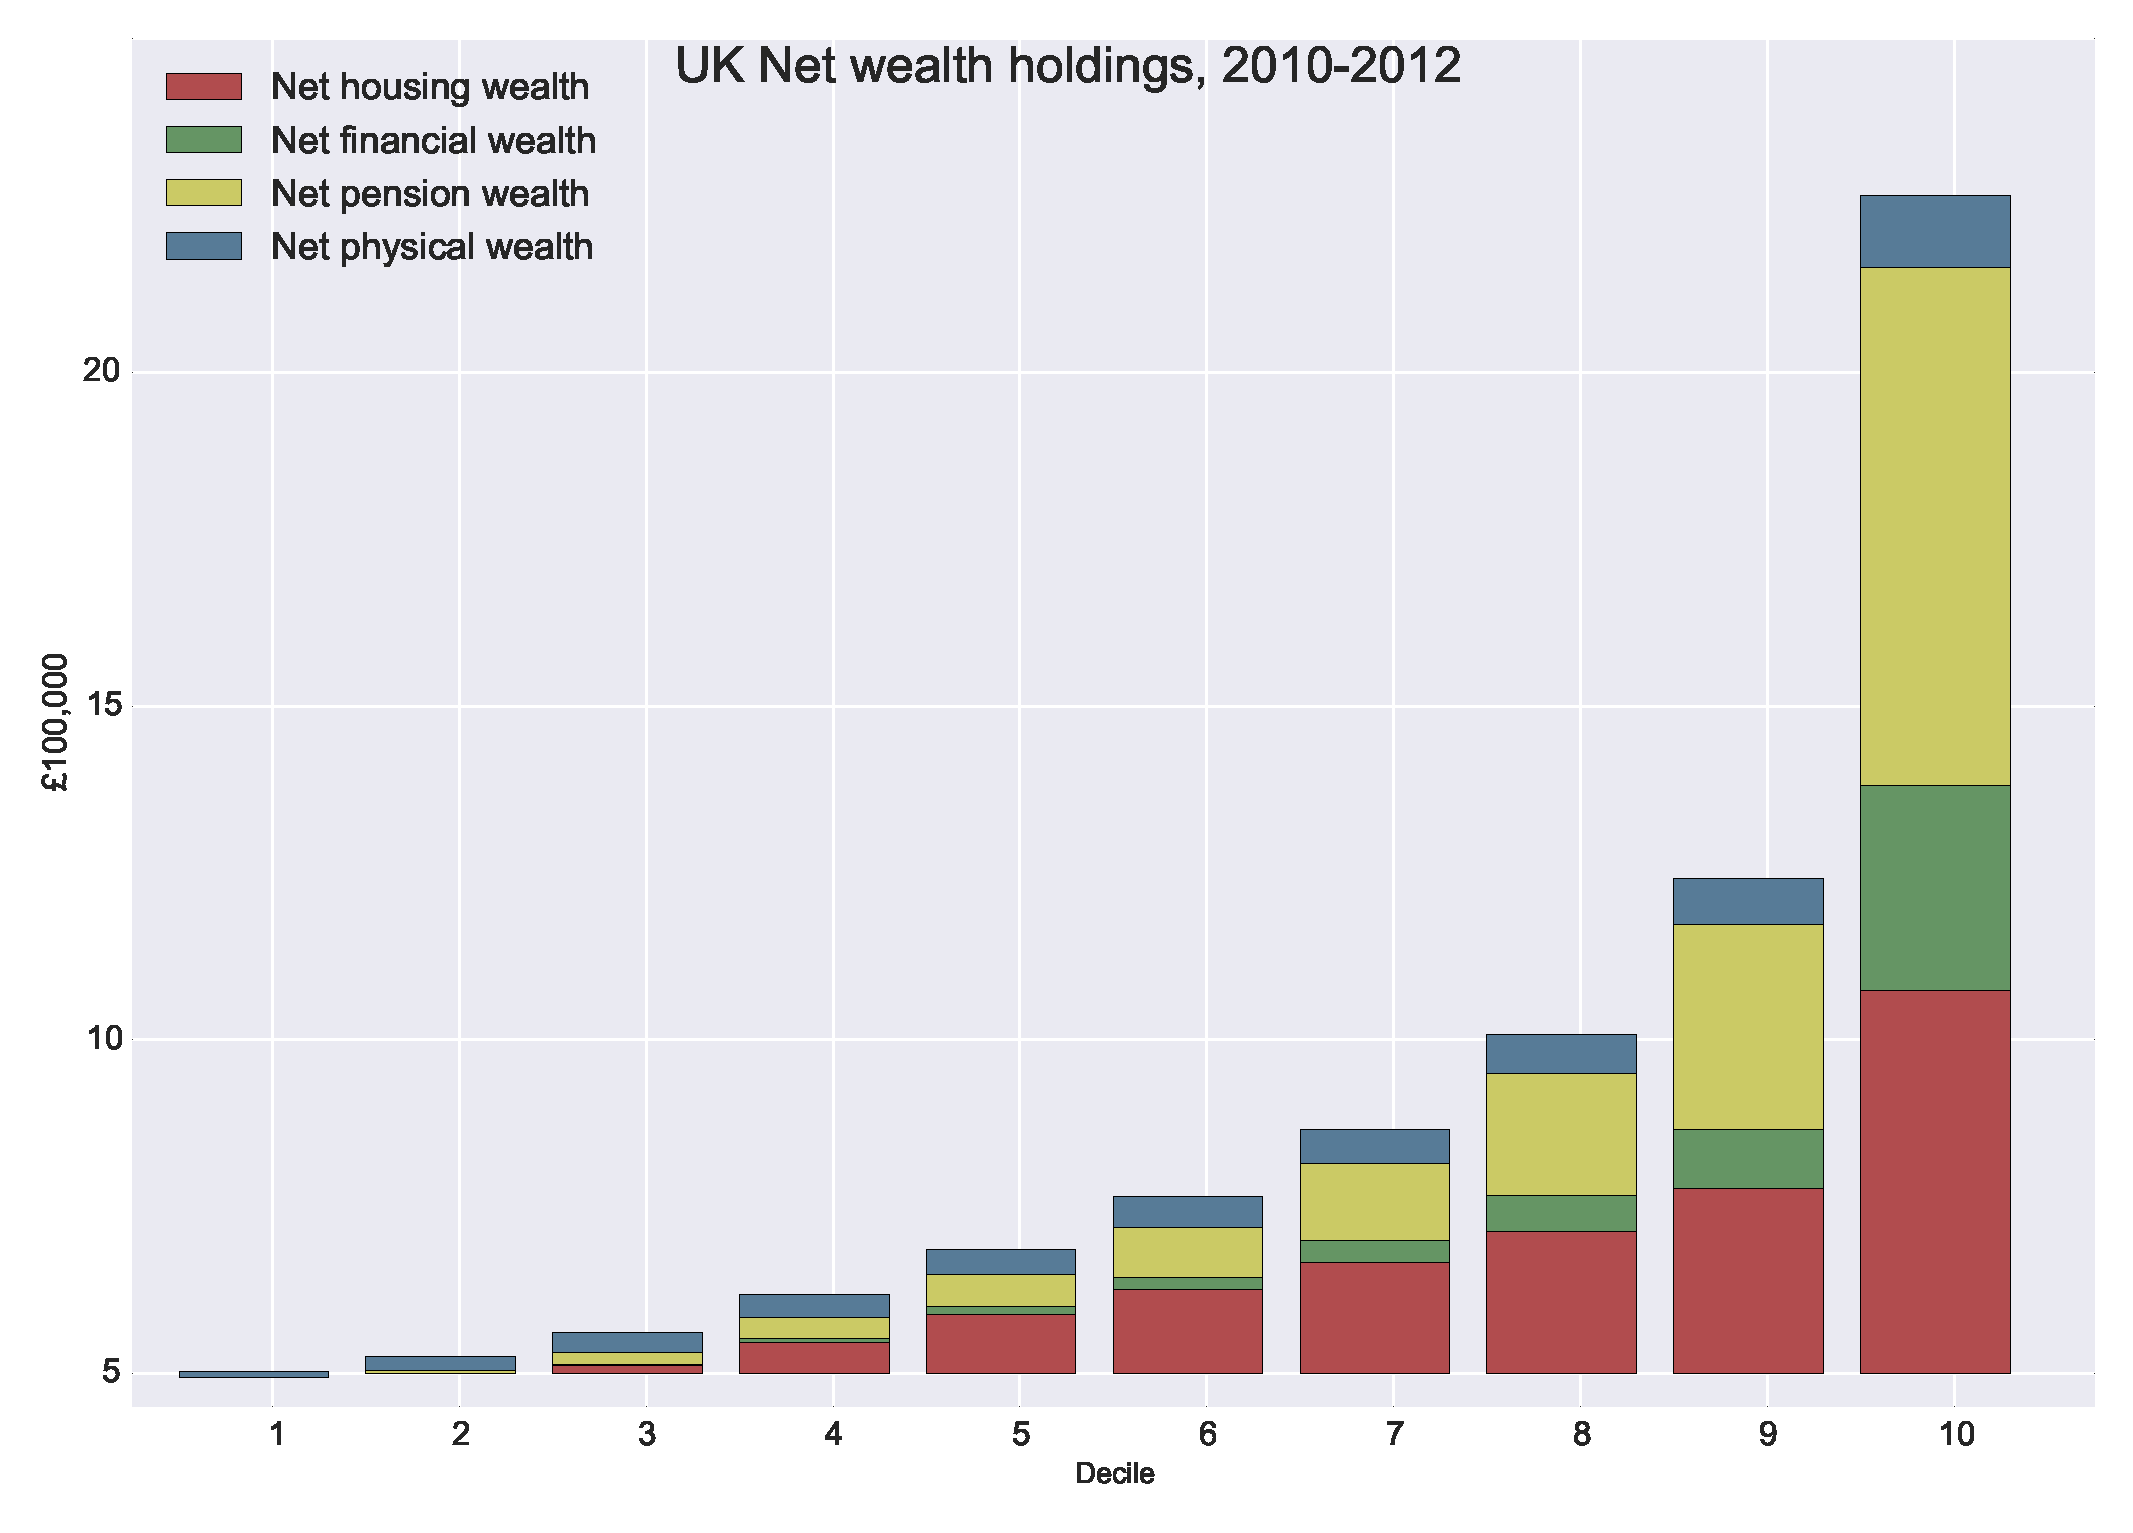
\includegraphics[width=\columnwidth]{was_wealth_holdings}
\caption{Histograms and cdfs of household net wealth in different data sets.}
\label{fig:was_wealthholdings}
\end{figure}

\section{A workhorse model}
The basic model underlying the discussion of savings behaviour and wealth 
accumulation in this chapter is the life-cycle model of household behaviour 
dating back to \citet{ModiglianiBrumberg1954} \footnote{A more detailed 
treatment of the general class of models can be found both in 
\citet{BrowningCrossley2001} and in \citet{AttanasioWeber2010}, although both 
papers have their focus on household consumption behaviour rather than wealth 
accumulation.}. The model can be written as a single household solving the 
problem

\begin{align}
\max_{\{c_{t+j}\}_{j=0}^{T-t}} \sum_{j=0}^{\infty} \delta^{t+j} \mathbb{E}_t \big[ u(c_{t+j}, z_{t+j}) \big] \label{maxprob}
\intertext{subject to} 
a_{t+1} = (1+r)(a_t + y_t - c_t) \label{bc}
\end{align}
where $T$ is the last period of the planning horizon, $\delta$ is the subjective
discount factor, $u()$ is the instantaneous felicity function -- usually assumed
to be of the CRRA form, $\frac{c^{1-\sigma}}{1-\sigma}$, where $\sigma$ is the 
coefficient of relative risk aversion --, $c$ is 
consumption, $a$ are financial assets, which allow the household to transfer 
resources across time, $r$ is a one-period interest rate, and $y$ is income. 
$z$ is used as a stand-in variable denoting the fact that households might, 
in general, care about other things that are not captured by the concept of 
current consumption; examples would be habits or durable consumption (which 
break the time-separability of the utility function), leisure time, particular 
classes of assets (such as housing) or bequests left to future generations.  
While in general, $T \rightarrow \infty$ is a possibility, and infinite horizon 
versions -- first advocated by \citet{Friedman1957} -- of the life-cycle model 
are widely used in macroeconomic applications, the finite horizon model will be 
more useful for the following discussion and forms the centrepiece of this 
thesis for a number of reasons which will become clear as we progress.

\section{Saving motives}
When trying to understand wealth distributions through the lens of the model
outlined above, the key question is: why do households save? The basic model,
in which consumers only care about the time path of instantaneous utility 
derived from consumption, suggests that households will save if and only if
it leads to preferential allocation of consumption over time -- they engage 
in consumption smoothing. As \citet{BrowningCrossley2001} point out, consumption
smoothing can happen at different frequencies, depending on the exact set-up 
of the model. In \citet{ModiglianiBrumberg1954} the main reason saving was the
existence of a retirement period, which necessitates consumption smoothing over
the life cycle -- wealth accumulation during working life to pay for consumption
in retirement. The implication of this simple model is that wealth accumulation
on the household level solely depends on the length of the retirement period, 
while in aggregate wealth accumulation crucially hinges on the growth rate
of the economy. The crucial assumption that allows Modigliani and Brumberg to
focus on consumption smoothing over the life cycle was that of constant income.


\section{Income uncertainty and market structure}
With the assumption of a non-constant income stream, it becomes important to 
think about the opportunities households have to insure themselves against
these fluctuations, or, in other words, which market structure they are facing.
To make income fluctuations relevant for the economic agent, the world of 
complete markets, in which a full set of Arrow securities covering each possible
state of the world can be bought and sold, has to be abandoned in favour of 
market \textit{incompleteness}. The most convenient, and at the same time most
extreme, departure from the complete markets assumption is to assume away any
sort of insurance markets except for very simple self-insurance through risk-
free one-period bonds. This market structure is implicit in the formulation of
the consumer problem in equation \ref{bc} -- there is just one asset for the 
household to sell or buy, and this asset has a certain payoff in the following 
period, which is not contingent on the state of the world. The big advantage of 
this setup is tractability: simple models of this kind can often be solved 
analytically, and in recursive formulations of more complex problems, the simple
market structure only adds one state variable to the problem. The drawback, 
obviously, is that this market structure is at odds with the economic reality,
where households are able to buy a hoist of different assets that vary widely 
in liquidity as well as in the degree to which payoff are state-contingent.
We defer the consideration of the role of liquidity to section \ref{housing}, 
which deals with the largest asset in most households' portfolio, housing, and
examine the role of insurance first. The basic idea when investigating the 
extent to which households have access to insurance mechanisms is to analyse
the joint dynamics of income and consumption data, and compare them with the
implications derived from models with different insurance mechanisms. In a 
complete market setup, where households can fully insure income risk, 
idiosyncratic changes in income should not translate into changes in consumption,
implying a flat profile of cross-sectional consumption inequality over the life-
cycle, irrespective of the underlying stochastic process governing income


\citet{BlundellPistaferriPreston2008}

\citet{KaplanViolante2010} examine how to what extent the empirical estimates
of consumption insurance that \citet{BlundellPistaferriPreston2008} obtain can
be replicated in a standard incomplete market model with capital as the only 
savings vehicle. 

\section{The role of housing}\label{housing}
While much effort has been devoted to examining the implications of income risk
and market structure for wealth accumulation through precautionary savings, it 
is undeniable that a large part of household saving happens in the form of an
asset which cannot perform the role of buffering against income shocks: housing.
As figure \ref{fig:was_wealthholdings} demonstrates using data from the US SCF and
the British Wealth and Asset Survey, by far the largest share of household
portfolios is invested in housing wealth, with the notable exception of the
very richest households. The illiquidity of housing, the high transaction costs
and the consumption element of housing purchases make this asset fundamentally
different from the one-period riskless bond considered in our workhorse model.
A number of authors have considered the effects of allowing households to save
in housing assets in addition to financial assets: \citet{CampbellHercovitz2009} 




\citet{CampbellHercovitz2005}
\citet{Yang2009}
\citet{Iacoviello2008}

\section{Closed and open economies}
On the endogeneity of interest rates

\section{Wealth Distribution Papers}
In the last years, many authors have used the increasing possibilities offered
by the increase in computing power to derive an additional implication from the
broad class of incomplete market models outlined above: a simulated wealth 
distribution. While there are many practical difficulties in creating model 
outputs that can reasonably compared to the data collected in surveys (some of
which have been alluded to in the above discussion on the definition of wealth),
in principle the simulated wealth distribution derived from life-cycle models
can be used to calibrate deep parameters of the model, provide an additional
test for how well the model is able to capture household savings behaviour, 
and shed light on which mechanisms are crucial in driving the evolution of 
aggregate savings at different parts of the distribution. \\
An early attempt to use the wealth distribution to estimate the parameters of
a life-cycle model of household savings can be found in \citet{Cagetti2003},
who uses a simple model similar to the one outlined in equations \ref{maxprob}
and \ref{bc}. Important additions in his version of the model are a bequest 
motive -- which, ceteris paribus, will increase the wealth holdings of elderly
households -- and a simplified pension system, which guarantees each household
a pension depending on their education level, and thereby lowers wealth 
accumulation during working life. The idea behind the estimation strategy is 
simple: given a stochastic process for household income, the parameters $\beta$,
$\sigma$ and $\alpha$ pin down a solution to the household's savings problem 
which allows one to simulate a theoretical wealth distribution from optimal 
household behaviour. Therefore, it is possible to use the simulated method of
moments to construct an estimator that chooses the triplet $(\delta,\sigma, 
\alpha)$ which minimises the distance between empirical moments of the wealth
distribution and its simulated counterparts. Given the high skewness of wealth
data, Cagetti opts for median wealth by 5-year age group as the moment to match.
As has become clear in the previous discussion, a crucial element driving 
household choices in the model is the income risk they face, making the choice
for the stochastic process representing this risk and its calibration a crucial
step in modelling wealth distributions. Cagetti opts for a process consisting
of a trend growth component common to all households, an age-education component
estimated for CEX data, and an MA(1) process representing the stochastic nature
of income. With his calibration, Cagetti finds low degrees of persistence, with
pronounced heterogeneity across education groups, and high degrees of risk 
aversion, implying a significant contribution of precautionary savings to 
aggregate wealth. \\
A very similar exercise is performed by \citet{HintermaierKoeniger2011}, who 
construct a minimum distance estimator based on the shape of the cross-sectional
distribution of wealth at different stages of the life cycle. That is, rather
than simply targeting the 50th percentile of wealth holdings  as 
\citet{Cagetti2003}, here all percentiles of the wealth distribution from 10 
to 90 are considered. The reason for excluding the upper ten percentiles of the
distribution are the well-known problems that a simple life-cycle model has in 
matching the extreme levels of wealth concentration observed at the upper end 
of the distribution, which might be driven by other motives than the buffer-
stock and retirement savings motives included in the model. Increasing the 
number of moments to match leads to estimates of the discount factor which are 
an order of magnitude more precise than in \citet{Cagetti2003}. The estimate for
the discount factor, at $\hat{\delta}=0.985$, is at the upper bound of the
estimates in \citet{Cagetti2003}, while the estimated risk aversion parameter
$\hat{\sigma}=1.08$ is only a third to one sixth as large as Cagetti's estimate,
depending on the subgroup under consideration.  


\citet{CastanedaRiosRull2003}
\citet{DPMRR2003}
\citet{Floden2008}
\citet{BenhabibBisinZhu2011}
\citet{DeNardiYang2015}

\section{Conclusion}
This chapter provides an overview of stylised facts about the wealth 
distributions in a number of advanced economies and presents various approaches 
to build economic models which can account for these stylised facts.
It became clear that while saving for retirement is the main driver of wealth
accumulation for large parts of the population, other factors need to be taken
into consideration to explain the tails of the distribution and the behaviour of
young households. Crucial aspects of an economic model of the wealth 
distribution are the risks households are facing -- both on the income and the 
expenditure side -- and the financial markets available to them to insure 
themselves against those risks and earn returns on their savings. Finally, the 
far right tail of the wealth distribution seems to be driven by factors beyond 
this and it is not clear whether variation in subjective discount factors, 
entrepreneurial activity, or other factors are best suited to model wealth 
accumulation at the top.
 